\documentclass{article}
\usepackage{neb-macros}
\usepackage{tikz}
  \usetikzlibrary{patterns}

\begin{document}

\CheapTitle{Quotient Rings and Ideals}

The difficult thing about coming up with a ring (really, the only thing) is defining the arithmetic operations, $+$ and $\cdot$, so that they satisfy all of the ring axioms. Rather than coming up with these operations out of whole cloth, if we already have some rings lying around we might try to build a new ring out of their ``parts''. We've already seen a few examples of exactly this idea.
\begin{itemize}
\item Subrings, built using subsets of existing rings
\item Direct sums, built using tuples with entries from existing rings
\item Localization, built out of fractions
\item Polynomial rings, matrix rings, rings of functions, and more.
\end{itemize}
Another way to build new rings out of the parts of old ones is by constructing \emph{quotients}. This idea is very frequently a stumbling block for beginning students of mathematics, so we will spend some time on it. But our effort will be rewarded; quotient rings turn out to be an extremely powerful and natural idea, and more generally the concept of ``quotient'' used here is pervasive in other fields of math.

Here is the basic idea behind quotient rings: given a ring $R$, partition $R$ into equivalence classes as $R/\Phi$. Now attempt to define an arithmetic on \emph{equivalence classes} as follows:
\begin{itemize}
\item Given two \emph{classes}, say $X$ and $Y$ in $R/\Phi$, \textbf{choose} some representatives $x \in X$ and $y \in Y$. Now compute the sum $x+y$ in $R$. This element is in some other class $Z$ in $R/\Phi$. We define $Z$ to be the sum of $X$ and $Y$.
\item Likewise, to multiply classes, we \textbf{choose} representatives, multiply in $R$, and determine the class of the product.
\end{itemize}

This is a fine idea, but unfortunately it has a problem: the sum of two classes may depend on our \textbf{choice} of representatives. See Figure \ref{fig:quot} for a graphic example. As a more concrete example, consider that the set of integers can be partitioned into two sets; the primes $P$ and the nonprimes $N$. We might try to compute the sum $P+P$ using representatives $2$ and $3$; in this case \[ P + P = [2] + [3] = [2+3] = [5] = P. \] But if we use representatives 3 and 7, we have \[ P + P = [3] + [7] = [3+7] = [10] = N. \] This is a problem- it means that this $+$ operation is not well-defined.

\begin{figure}[h]
\begin{center}
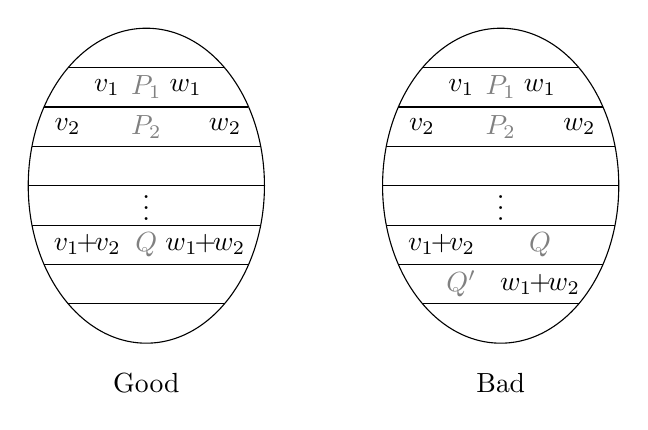
\begin{tikzpicture}[scale=0.5]
  \draw (3,4) ellipse (3 and 4);
  \draw (1.02,1) edge (4.98,1);
  \draw (0.40,2) edge (5.59,2);
  \draw (0.09,3) edge (5.90,3);
  \draw (0.00,4) edge (6.00,4);
  \draw (0.09,5) edge (5.90,5);
  \draw (0.40,6) edge (5.59,6);
  \draw (1.02,7) edge (4.98,7);
  \node at (3,3.65) {$\vdots$};
  \node at (2,6.5) {$v_1$};
  \node at (4,6.5) {$w_1$};
  \node at (1,5.5) {$v_2$};
  \node at (5,5.5) {$w_2$};
  \node at (1.5,2.5) {$v_1\!\!+\!\!v_2$};
  \node at (4.5,2.5) {$w_1\!\!+\!\!w_2$};
  \node at (3,6.5) [gray] {$P_1$};
  \node at (3,5.5) [gray] {$P_2$};
  \node at (3,2.5) [gray] {$Q$};
  \node at (3,-1) {Good};
  
  \draw (12,4) ellipse (3 and 4);
  \draw (10.02,1) edge (13.98,1);
  \draw (09.40,2) edge (14.59,2);
  \draw (09.09,3) edge (14.90,3);
  \draw (09.00,4) edge (15.00,4);
  \draw (09.09,5) edge (14.90,5);
  \draw (09.40,6) edge (14.59,6);
  \draw (10.02,7) edge (13.98,7);
  \node at (12,3.65) {$\vdots$};
  \node at (11,6.5) {$v_1$};
  \node at (13,6.5) {$w_1$};
  \node at (10,5.5) {$v_2$};
  \node at (14,5.5) {$w_2$};
  \node at (10.5,2.5) {$v_1\!\!+\!\!v_2$};
  \node at (13,1.5) {$w_1\!\!+\!\!w_2$};
  \node at (12,6.5) [gray] {$P_1$};
  \node at (12,5.5) [gray] {$P_2$};
  \node at (13,2.5) [gray] {$Q$};
  \node at (11,1.5) [gray] {$Q^\prime$};
  \node at (12,-1) {Bad};
\end{tikzpicture}
\caption{\label{fig:quot}What can go wrong when making partitions into rings}
\end{center}
\end{figure}

To fix this problem, we just need to make sure our partition is chosen so that this bad thing never happens.

\begin{dfn}[Ring Congruence]
Let $R$ be a ring. An equivalence relation $\Phi$ on $R$ is called a \emph{congruence} if the following hold.
\begin{enumerate}
\item If $x_1 \Phi y_1$ and $x_2 \Phi y_2$, then $(x_1+x_2) \Phi (y_1+y_2)$.
\item If $x_1 \Phi y_1$ and $x_2 \Phi y_2$, then $(x_1 \cdot x_2) \Phi (y_1 \cdot y_2)$.
\end{enumerate}
\end{dfn}

\begin{prop}
If $\Phi$ is a congruence on a ring $R$ and $x \Phi y$ then $(-x)\Phi(-y)$.
\end{prop}

\begin{proof}
We have $x \Phi y$, $(-x) \Phi (-x)$, and $(-y) \Phi (-y)$. So $(x-x-y)\Phi(y-x-y)$, and thus $(-y)\Phi(-x)$, so that $(-x)\Phi(-y)$.
\end{proof}

\begin{prop}
Let $R$ be a ring and $\Phi$ an equivalence on $R$.
\begin{enumerate}
\item The operations $+$ and $\cdot$ on $R/\Phi$ given by \[ [a] + [b] = [a+b] \quad \mathrm{and} \quad [a] \cdot [b] = [a \cdot b] \] are well-defined if and only if $\Phi$ is a congruence.
\item In this case, $(R/\Phi, +, \cdot)$ is a ring, called the \emph{quotient} of $R$ by $\Phi$. If $R$ is commutative, then $R/\Phi$ is commutative, and if $R$ is unital, the $R/\Phi$ is unital.
\end{enumerate}
\end{prop}

\begin{proof}
(type this)
\end{proof}

The congruence condition may at first glance seem to be very strong -- so strong that we might doubt whether any such equivalences exist. We will see that they are abundant. In fact, we already know of one very important example: $\ZZ/(n)$ is the quotient of $\ZZ$ by the congruence $r \Phi s \Leftrightarrow n|(s-r)$. More generally,

\begin{prop}
Let $R$ be a commutative ring and $a \in R$. The relation $\Phi$ on $R$ given by $r \Phi s$ iff $a | (s-r)$ is a congruence. We denote the ring $R/\Phi$ by $R/(a)$.
\end{prop}

\begin{proof}
(exercise.)
\end{proof}

As an example, what can we say about the ring $\QQ[x]/(x^2 + 1)$? Using the division algorithm, every polynomial in $\QQ[x]$ can be written as $(x^2+1)q(x) + r(x)$, where $r$ is either 0, a nonzero constant, or a linear polynomial. Etc. etc.

\subsection*{What are congruences?}

We've seen that special equivalence relations called \emph{congruences} can be used to build new rings out of old ones via the quotient construction. We'd like to understand the congruences in more depth.

\begin{prop}
Let $R$ be a ring and $\Phi$ a congruence on $R$. Let $I$ be the $\Phi$-class of 0.
\begin{enumerate}
\item $I$ is a subring of $R$.
\item $I$ absorbs $R$ under multiplication from either side. That is, if $a \in I$ and $r \in R$, then $ar \in I$ and $ra \in I$.
\item Every $\Phi$-class is of the form $r + I = \{ r+a \mid a \in I \}$ for some $r \in R$. Sets of this form are called \emph{cosets}.
\end{enumerate}
\end{prop}

\begin{dfn}[Ideal]
Let $R$ be a ring. A subring $I \subseteq R$ which absorbs $R$ under multiplication from both sides is called an \emph{ideal}. 
\end{dfn}

\begin{prop}
Let $R$ be a ring and $\Phi$ an equivalence on $R$. Then the following are equivalent.
\begin{enumerate}
\item $\Phi$ is a congruence.
\item There is an ideal $I \subseteq R$ such that the $\Phi$-classes are precisely the cosets of $I$.
\item There is a surjective ring homomorphism $\varphi : R \rightarrow S$ such that $x \Phi y$ if and only if $y-x \in \KER{\varphi}$.
\end{enumerate}
\end{prop}

\begin{proof}
(type this)
\end{proof}

That is, the congruences on a ring are in bijective correspondence with special subsets called \emph{ideals}. It is much easier to directly describe ideals in a ring than congruences (although the two are equivalent). For this reason, if $\Phi$ is a congruence with associated ideal $I$, we will frequently abuse the notation and refer to the quotient ring $R/I$ rather than $R/\Phi$, with the understanding that $R/I$ is the quotient with respect to the congruence $y-x \in I$.

\subsection*{The First Isomorphism Theorem}

Defining a mapping on a quotient set is generally difficult, for the same reason that defining operations on a quotient set is difficult; the most natural thing to try is to define our mapping in terms of representatives, but this is generally not well-defined.

The first important result about quotient rings gives us a standard way to construct homomorphisms on a quotient ring that bypasses this difficulty. This result, known as the First Isomorphism Theorem, is due to Emmy Noether, and is an important tool in ring theory.

\begin{prop}[First Isomorphism Theorem for Rings]
Let $R$ be a ring and $I$ an ideal of $R$.
\begin{enumerate}
\item The natural projection $\pi : R \rightarrow R/I$ given by $\pi(x) = x+I$ is a ring homomorphism, which is unital if $R$ is unital.
\item If $\varphi : R \rightarrow S$ is a ring homomorphism such that $I \subseteq \KER{\varphi}$, then there is a ring homomorphism $\overline{\varphi} : R/I \rightarrow S$ such that $\overline{\varphi}(x + I) = \varphi(x)$. That is, $\varphi = \overline{\varphi} \circ \pi$.
\end{enumerate}
\end{prop}

Another way to state FIT is as follows: If $\varphi$ is a ring homomorphism and $I$ an ideal contained in the kernel of $\varphi$, then $\varphi$ factors through the projection induced by $I$. This terminology is inspired by the commutative diagram associated to FIT, in which we literally have $\varphi = \overline{\varphi} \circ \pi$.

\subsection*{Exercises}

\begin{enumerate}
\item (One-sided ideals)
\end{enumerate}

\end{document}
